\documentclass[12pt,a4paper]{report}
\usepackage[T1]{fontenc}
\usepackage[utf8]{inputenc}
\usepackage[a4paper,margin=1in]{geometry}
\usepackage{setspace}
\usepackage{lmodern}
\usepackage{microtype}
\usepackage{graphicx}
\usepackage{booktabs}
\usepackage{array}
\usepackage{longtable}
\usepackage{float}
\usepackage{hyperref}
\usepackage{enumitem}
\usepackage{caption}
\usepackage[svgnames]{xcolor}
\usepackage{titlesec}
\usepackage{fancyhdr}
\usepackage{ragged2e}
\usepackage{tikz}
\usetikzlibrary{arrows.meta,positioning,shapes.geometric}

\linespread{1.18}
\setlength{\parskip}{0.55em}
\setlength{\parindent}{0pt}
\setlength{\headheight}{15pt}
\renewcommand{\arraystretch}{1.22}
\captionsetup{font=small,labelfont=bf}

\hypersetup{
    colorlinks=true,
    linkcolor=MidnightBlue,
    urlcolor=MidnightBlue,
    citecolor=MidnightBlue,
    pdftitle={Blood Cancer Detection Using a Multilevel Hierarchical Deep Learning Pipeline}
}

\titleformat{\section}
    {\Large\bfseries\color{MidnightBlue}}
    {}
    {0pt}
    {}

\titlespacing*{\section}{0pt}{1.2em}{0.6em}

\pagestyle{fancy}
\fancyhf{}
\fancyhead[L]{Blood Cancer Detection Report}
\fancyhead[R]{\thepage}
\fancyfoot[C]{IIIT Raichur}

\newcommand{\templchapter}[1]{%
    \section*{#1}%
    \addcontentsline{toc}{section}{#1}%
}

\begin{document}
\justifying

\begin{titlepage}
\begin{center}
\vspace*{0.8cm}

{\Large \textbf{Project Report}}\\[0.8cm]

\rule{0.85\textwidth}{0.8pt}\\[0.5cm]
{\Huge \textbf{Blood Cancer Detection Using a}}\\[0.25cm]
{\Huge \textbf{Multilevel Hierarchical Deep Learning Pipeline}}\\[0.5cm]
\rule{0.85\textwidth}{0.8pt}\\[0.9cm]

{\large by}\\[0.6cm]

{\Large \textbf{Theegala Yeseswini}}\\[0.15cm]
{\large AD25B1035}\\[0.9cm]

{\large Independent Project}\\[0.2cm]
{\large Artificial Intelligence and Data Science}\\[0.6cm]

{\large Indian Institute of Information Technology Raichur (IIITR)}\\[0.2cm]
{\large Raichur, Karnataka -- 584135}\\[0.9cm]

{\large 2026}

\vfill
\end{center}
\end{titlepage}

\fancyhead[L]{Contents}
\pagenumbering{roman}
\tableofcontents
\clearpage

\fancyhead[L]{Blood Cancer Detection Report}
\pagenumbering{arabic}

\templchapter{ABSTRACT}
This project presents a deep learning based blood cancer image classification system built on microscopic blood-smear images. Instead of solving the full problem with a single flat classifier, the proposed system follows a multilevel hierarchical pipeline. In the first level, a broad disease classifier categorizes each image into one of four groups: leukemia, lymphoma, myeloma, or healthy. In the second level, specialized subtype classifiers are triggered only when the broad model predicts leukemia or lymphoma. The leukemia branch further classifies the sample into ALL, AML, CLL, or CML, while the lymphoma branch predicts CLL, FL, or MCL.

This design was chosen because the datasets are highly imbalanced and the subtype labels are not equally difficult. A single model must learn both coarse disease separation and fine-grained subtype discrimination at the same time, which increases confusion, especially for visually similar or rare classes. The hierarchical approach reduces this burden by first solving a simpler high-level task and then delegating difficult subtype recognition to dedicated expert models. It also improves interpretability because the final output follows a clear clinical-style path: disease family first and subtype next.

The implemented system combines an EfficientNet-B0 broad classifier, an EfficientNet-B0 leukemia subtype classifier, and a DenseNet121 lymphoma subtype classifier. The broad classifier achieved 99.79\% test accuracy, the leukemia subtype classifier achieved 87.62\% test accuracy, and the lymphoma subtype classifier achieved 84.00\% validation accuracy. A flat single-stage baseline produced only 78.53\% test accuracy and 71.29\% weighted F1-score. These results show that the proposed multilevel pipeline is a more reliable and structured solution for this task.

\templchapter{INTRODUCTION}
Blood cancer detection from microscopic imagery is an important and challenging image classification problem because the visual differences between disease categories and their subtypes can be subtle. Manual screening is time-consuming and depends heavily on expert interpretation, so computer-aided systems can help by providing faster and more consistent preliminary predictions. In this work, deep convolutional neural networks are used to classify blood cell images into disease categories and finer disease subtypes.

The project focuses on four broad outcomes: leukemia, lymphoma, myeloma, and healthy. However, the underlying medical problem is naturally hierarchical rather than flat. Leukemia and lymphoma each contain multiple subtype labels, and some labels are visually harder than others because of limited data and class overlap. For that reason, the project adopts a routed inference strategy where a broad model first determines the disease family, and only then a specialized subtype model is invoked when needed. This makes the system closer to the real problem structure and easier to interpret during deployment.

\templchapter{AIM, MOTIVATION, and OBJECTIVES}
\textbf{Aim:} To develop an accurate and interpretable deep learning system for blood cancer detection and subtype classification from microscopic blood cell images.

\textbf{Motivation:} A direct multiclass model struggles when the data contains class imbalance, visually similar categories, and repeated subtype names across different disease families. A hierarchical pipeline offers better task decomposition, easier debugging, and a clearer prediction path for users.

\textbf{Objectives:}
\begin{itemize}[leftmargin=1.5em]
    \item Build a broad classifier to separate leukemia, lymphoma, myeloma, and healthy cases.
    \item Train a dedicated leukemia subtype classifier for ALL, AML, CLL, and CML.
    \item Train a dedicated lymphoma subtype classifier for CLL, FL, and MCL.
    \item Compare the proposed multilevel approach with a flat single-stage baseline.
    \item Present the final system through a reproducible inference pipeline and report.
\end{itemize}

\templchapter{PROPOSED METHODOLOGY}
\textbf{Dataset composition:} The broad classifier was built from combined microscopy datasets representing leukemia, lymphoma, myeloma, and healthy classes. The approximate image counts observed in the notebooks were 12000 leukemia images, 374 lymphoma images, 498 myeloma images, and 3000 healthy images. The lymphoma images were oversampled by a factor of 4 and the myeloma images by a factor of 2 to reduce class imbalance.

\textbf{Preprocessing:} Input images were converted to RGB, resized to $224 \times 224$, and normalized before inference. Training used data augmentation such as horizontal flips, rotations, color jitter, random resized crops, Gaussian blur, and grayscale transforms depending on the model branch.

\textbf{Model architecture:}
\begin{itemize}[leftmargin=1.5em]
    \item Broad classifier: EfficientNet-B0
    \item Leukemia subtype classifier: EfficientNet-B0
    \item Lymphoma subtype classifier: DenseNet121
\end{itemize}

\textbf{Multilevel hierarchical pipeline:} The first level predicts the broad disease family. If the result is leukemia, the sample is forwarded to the leukemia subtype model. If the result is lymphoma, the sample is forwarded to the lymphoma subtype model. If the result is myeloma or healthy, the broad prediction itself becomes the final output.

\begin{figure}[H]
\centering
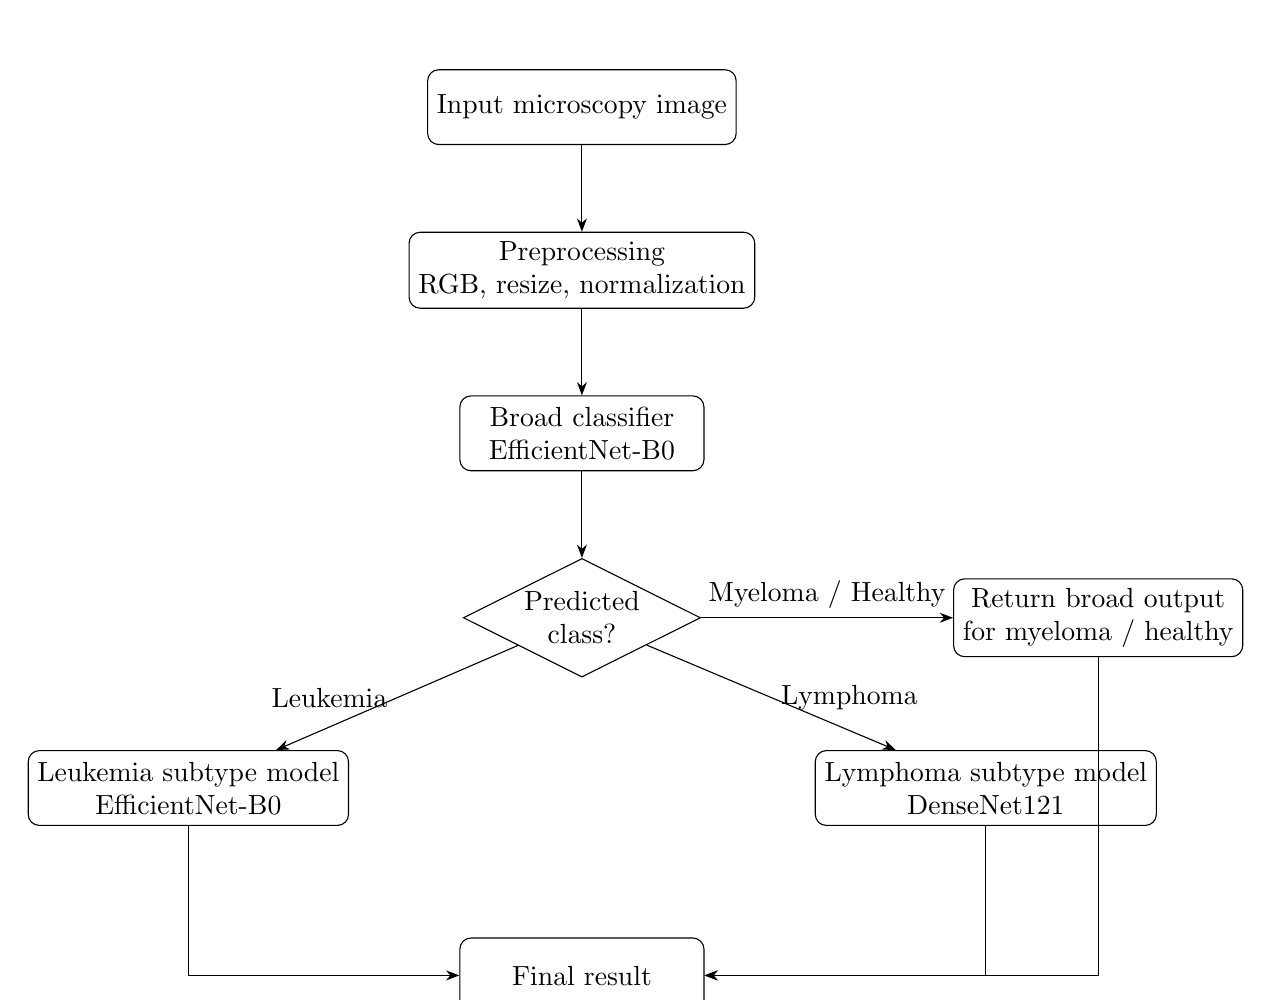
\begin{tikzpicture}[
    node distance=1.1cm and 1.5cm,
    box/.style={draw, rounded corners, align=center, minimum width=3.1cm, minimum height=0.95cm},
    decision/.style={draw, diamond, aspect=2, align=center, inner sep=1pt},
    >=Stealth
]
\node[box] (input) {Input microscopy image};
\node[box, below=of input] (prep) {Preprocessing\\RGB, resize, normalization};
\node[box, below=of prep] (broad) {Broad classifier\\EfficientNet-B0};
\node[decision, below=of broad] (route) {Predicted\\class?};
\node[box, below left=1.3cm and 2.2cm of route] (leuk) {Leukemia subtype model\\EfficientNet-B0};
\node[box, below right=1.3cm and 2.2cm of route] (lymph) {Lymphoma subtype model\\DenseNet121};
\node[box, below=3.3cm of route] (final) {Final result};
\node[box, right=3.2cm of route] (direct) {Return broad output\\for myeloma / healthy};

\draw[->] (input) -- (prep);
\draw[->] (prep) -- (broad);
\draw[->] (broad) -- (route);
\draw[->] (route) -- node[left] {Leukemia} (leuk);
\draw[->] (route) -- node[right] {Lymphoma} (lymph);
\draw[->] (route) -- node[above] {Myeloma / Healthy} (direct);
\draw[->] (leuk) |- (final);
\draw[->] (lymph) |- (final);
\draw[->] (direct) |- (final);
\end{tikzpicture}
\caption{Inference flow of the proposed multilevel hierarchical pipeline.}
\end{figure}

\textbf{Why the multilevel hierarchical pipeline was chosen:}
\begin{itemize}[leftmargin=1.5em]
    \item It decomposes a difficult 9-class problem into simpler decisions.
    \item It handles class imbalance better by isolating rare subtype learning inside dedicated models.
    \item It reduces confusion caused by overlapping subtype names such as CLL appearing in both leukemia and lymphoma contexts.
    \item It improves interpretability because the system explains both the broad disease family and the subtype route.
    \item It is modular, so each branch can be improved independently without retraining the entire system.
\end{itemize}

\templchapter{RESULTS}
Table~\ref{tab:stage-results} summarizes the performance of the proposed hierarchical pipeline at each level.

\begin{table}[H]
\centering
\caption{Stage-wise performance of the proposed system}
\label{tab:stage-results}
\begin{tabular}{>{\raggedright\arraybackslash}p{5.2cm} >{\raggedright\arraybackslash}p{4.5cm} >{\centering\arraybackslash}p{3cm}}
\toprule
\textbf{Model} & \textbf{Evaluation setting} & \textbf{Result} \\
\midrule
Broad disease classifier & 4-class test set & 99.79\% accuracy \\
Leukemia subtype classifier & 4-class subtype test set & 87.62\% accuracy \\
Lymphoma subtype classifier & 3-class validation split & 84.00\% accuracy \\
\bottomrule
\end{tabular}
\end{table}

The next comparison contrasts the proposed routed architecture with the flat single-stage baseline from \texttt{singleclassifier.ipynb}.

\begin{table}[H]
\centering
\caption{Comparison between flat baseline and proposed hierarchical approach}
\label{tab:baseline-compare}
\begin{tabular}{>{\raggedright\arraybackslash}p{4.2cm} >{\centering\arraybackslash}p{2.5cm} >{\centering\arraybackslash}p{2.7cm} >{\raggedright\arraybackslash}p{4.3cm}}
\toprule
\textbf{Approach} & \textbf{Accuracy} & \textbf{Weighted F1} & \textbf{Observation} \\
\midrule
Single-stage classifier & 78.53\% & 71.29\% & Direct 9-class prediction struggled on rare and visually similar classes \\
Hierarchical broad stage & 99.79\% & 99.79\% & Excellent coarse disease separation before routing \\
Hierarchical subtype branches & 87.62\% / 84.00\% & Branch-wise class F1s improved for difficult subtypes & Specialized models performed better on fine-grained recognition \\
\bottomrule
\end{tabular}
\end{table}

\textbf{Class-wise comparison:} The flat baseline was especially weak on difficult subtypes, while the routed models improved subtype recognition after disease-family separation.

\begin{table}[H]
\centering
\caption{Selected class-wise F1 comparison}
\label{tab:f1-compare}
\begin{tabular}{>{\raggedright\arraybackslash}p{3.5cm} >{\centering\arraybackslash}p{3cm} >{\centering\arraybackslash}p{3.5cm}}
\toprule
\textbf{Class} & \textbf{Flat baseline F1} & \textbf{Hierarchical branch F1} \\
\midrule
ALL & 0.00 & 0.76 \\
AML & 0.72 & 0.85 \\
Leukemia CLL & 0.86 & 0.90 \\
CML & 0.92 & 0.97 \\
Lymphoma CLL & 0.43 & 0.83 \\
FL & 0.69 & 0.90 \\
MCL & 0.45 & 0.77 \\
\bottomrule
\end{tabular}
\end{table}

\textit{Note:} The flat baseline is an end-to-end 9-class evaluation, whereas the proposed method is reported stage-wise because the subtype models are evaluated after routing. Even with this caveat, the class-wise subtype improvements strongly support the hierarchical design.

\templchapter{DISCUSSION}
The results show that the proposed multilevel hierarchical pipeline is a stronger and more meaningful solution than a flat single-stage model for this project. The broad classifier achieved 99.79\% accuracy, which means the first routing decision is highly reliable. This is important because the quality of the second-level subtype prediction depends on correct family-level separation.

The comparison with the single-stage baseline explains why the hierarchical design was preferred. The flat model achieved only 78.53\% test accuracy and 71.29\% weighted F1-score, with severe failure on some difficult classes such as ALL and lymphoma-related subtypes. In contrast, the routed models substantially improved subtype performance after narrowing the problem space. This happens because each branch learns a smaller and more consistent visual task instead of being forced to separate all disease categories at once.

Another major reason for selecting the hierarchical pipeline is label ambiguity. In the dataset, CLL appears in both leukemia and lymphoma branches, which makes a flat prediction space harder to learn. The multilevel design resolves that issue by first deciding the disease family and then assigning the subtype inside the correct branch. This improves interpretability, reduces confusion, and makes the output easier to justify in a project presentation.

\templchapter{CONCLUSION}
This work demonstrates that blood cancer image classification benefits from task decomposition. The proposed system first predicts the broad disease family and then performs subtype recognition only when necessary. The method achieved strong stage-wise performance, with 99.79\% broad classification accuracy, 87.62\% leukemia subtype accuracy, and 84.00\% lymphoma subtype accuracy.

The comparison with the single-stage baseline shows why the multilevel hierarchical approach is more suitable for this project. It gives better structure, stronger subtype discrimination, and clearer reasoning for the final prediction path. Future work can include external test-set evaluation for all branches, Grad-CAM based explainability, better lymphoma data balancing, and a fully modular training pipeline outside notebooks.

\templchapter{REFERENCES}
\begin{thebibliography}{9}

\bibitem{efficientnet}
Mingxing Tan and Quoc V. Le,
\textit{EfficientNet: Rethinking Model Scaling for Convolutional Neural Networks},
Proceedings of the 36th International Conference on Machine Learning, 2019.

\bibitem{densenet}
Gao Huang, Zhuang Liu, Laurens van der Maaten, and Kilian Q. Weinberger,
\textit{Densely Connected Convolutional Networks},
Proceedings of the IEEE Conference on Computer Vision and Pattern Recognition, 2017.

\bibitem{pytorch}
Adam Paszke et al.,
\textit{PyTorch: An Imperative Style, High-Performance Deep Learning Library},
Advances in Neural Information Processing Systems, 2019.

\bibitem{who}
World Health Organization,
\textit{Haematolymphoid Tumours: WHO Classification of Tumours},
WHO Classification of Tumours Editorial Board.

\bibitem{datasetnote}
Project notebooks and dataset configurations used in this work:
\texttt{Broadclassifier.ipynb}, \texttt{lukemia\_sub.ipynb}, \texttt{lymphoma\_sub.ipynb}, and \texttt{singleclassifier.ipynb}.

\end{thebibliography}

\end{document}
